The work presented here contributes to a compositional theory of ``co-design'' that allows to optimally design a robotic platform.
In this framework, a user models each subsystem as a monotone relation between \F{functionality provided} and \R{resources required}.
These models can be easily composed to express the co-design constraints between different subsystems.
The user then queries the model, to obtain the design with minimal resources usage, subject to a lower bound on the provided functionality.
This paper concerns the introduction of uncertainty in the framework.
Uncertainty has two roles: first, it allows to deal with limited knowledge in the models; second, it also can be used to generate consistent relaxations of a problem, as the computation requirements can be lowered should the user accept some uncertainty in the answer.

\section{Introduction}

The design of a robotic platform involves the choice and configuration of many hardware and software subsystems (actuation, energetics, perception, control, \dots) in an harmonious entity in which all \emph{co-design constraints} are respected.
Because robotics is a relatively young discipline, there is still little work towards obtaining systematic procedures to derive optimal designs.
Therefore, robot design is a lengthly design process mainly based on empirical evaluation and trial and error.
The work presented here contributes to a theory of co-design that allows to optimally design a robotic platform based on formal models of the performance of its subsystems.
The goal is to allow a designer to create better designs, faster.
This paper describes the introduction of uncertainty in the theory.

\subsubsection*{Previous work}

In previous work~\cite{censi15monotone,censi15same,censi16codesign_sep16},
I have proposed a compositional theory for co-design.
The user defines ``design problems'' (DPs) that describe the constraints for each subsystem.
These DPs can then be hierarchically composed and interconnected to obtain the class of Monotone Co-Design Problems (MCDPs).

An example of MCDP is sketched in~\cref{fig:Example1}.
The design problem consists in finding an optimal configuration of a UAV, optimizing over actuators, sensors, processors, and batteries.
Each design problem (DP) is formalized as a relation between \F{functionality}
and \R{resources}.
For example, the functionality of the UAV is parameterized by three numbers: the \F{distance to travel} for each mission; the \F{payload to transport}; the \F{number of missions} to fly.
The optimal design is defined as the one that satisfies the functionality constraints while using the minimal amount of \R{resources} (\R{cost} and \R{mass}).

The convenience of the MCDP framework is that the user can define design problems for each subsystem and then compose them.
The definition of the DPs is specified using a domain-specific language that promotes composition and code reuse; the formal specification is contained in the supplementary materials.
In the figure, the model is exploded to show how actuation and energetics are modeled.
Perception is modeled as a relation between \F{the velocity of the platform} and the \R{power} required.
Actuation is modeled as a relation between \F{lift} and \R{power}/\R{cost}.
Batteries are described by a relation between \F{capacity} and \R{mass}/\R{cost}.
The interconnection between these describe the ``co-design constraints'':\eg , actuators must lift the batteries, the batteries must power the actuators.
In this example, there are different battery technologies (LiPo, \etc), each specified by specific energy, specific cost, and lifetime, thus characterized by a different relation between \F{capacity}, \F{number of missions} and \R{mass} and \R{cost}.

Once the model is defined, it can be queried to obtain the \emph{minimal} solution in terms of resources \textemdash{} here, \R{total cost} and \R{total mass}.
The output to the user is the Pareto front containing all non-dominated solutions.
The corresponding optimization problem is, in general, nonconvex.
Yet, with few assumptions, it is possible to obtain a systematic solution procedure, and show that there exists a dynamical system whose fixed point corresponding to the set of minimal solutions.

\subsubsection*{Contribution}

This paper describes how to add a notion of \emph{uncertainty} in the MCDP framework.
The model of uncertainty considered is interval uncertainty on arbitrary partial orders.
For a poset~$\left\langle \posA,\posleq\right\rangle $, these are sets of the type~$\{x\setin\posA\colon a\posleq x\posleq b\}$.
I will show how one can introduce this type of uncertainty in the MCDP framework by considering ordered pairs of design problems.
Each pair describes lower and upper bounds for resources usage.
These \emph{uncertain design problems} (UDPs) can be composed using series, parallel, and feedback interconnection, just like their non-uncertain counterparts.

The user is then presented with \emph{two} Pareto fronts, corresponding to a lower bound and an upper bound for resource consumption, in the best case and in the worst case, respectively.

This is different from the usual formalization of ``robust optimization''~(see \eg , \cite{bertsimas11theory,ben-tal09}), usually formulated as a ``worst case'' analysis, in which one the uncertainty in the problem is described by a set of possible parameters, and the optimization problem is posed as finding the one design that is valid for all cases.

Uncertainty plays two roles: it can be used as a \emph{modeling} \emph{tool}, where the relations are uncertain because of our limited knowledge, and it can be used as a \emph{computational} \emph{tool}, in which we deliberately choose to consider uncertain relations as a relaxation of the problem, to reduce the computational load, while maintaining precise consistency guarantees.
With these additions, the MCDP framework allows to describe even richer design problems and to efficiently solve them.

\subsubsection*{Paper organization}

%\Cref{sec:Design-Problems} and \ref{sec:Monotone-Co-Design-Problems}
%summarize previous work.

They give a formal definition of design problems
(DPs) and their composition, called Monotone Co-Design Problems (MCDPs).
\Cref{sec:UDP} through~\cref{sec:Approximation-results} describe the notion of Uncertain Design Problem (UDP), the semantics of their interconnection, and the general theoretical results.
\Cref{sec:Applications} describes three specific applications of the theory with numerical results.
The supplementary materials include detailed models written in MCDPL and pointers to obtain the source code and a virtual machine for reproducing the experiments.

\section{Design Problems}

\emph{A design problem} (DP) is a monotone relation between \emph{\F{provided functionality}} and \emph{\R{required resources}}. \F{Functionality} and \R{resources} are complete partial orders (CPO)~\cite{davey02}, indicated by~$\langle\funsp,\posleqof{\funsp}\rangle$ and~$\langle\ressp,\posleqof{\ressp}\rangle$.
The graphical representations uses nodes for DPs and green (red) edges for \F{functionality} and \R{resources}~(\cref{fig:dp}).

\captionsideleft{\label{fig:dp}}{\includegraphics[scale=0.33]{unc_dpcartoon}}
\begin{example}
    The first-order characterization of a battery is as a store of energy, in which the \F{capacity {[}kWh{]}} is the \F{functionality} (what the battery provides) and \R{mass} {[}kg{]} and \R{cost} {[}\${]} are \R{resources} (what the battery requires)~(\cref{fig:battery1}).
\end{example}
\captionsideleft{\label{fig:battery1}}{\includegraphics[scale=0.33]{unc_battery_masscost}}

In general, fixed a functionality~$\fun\setin\funsp$, there will be multiple resources in~$\ressp$ sufficient to perform the functionality that are incomparable with respect to~$\posleqof{\ressp}$.
For example, in the case of a battery one might consider different battery technologies that are incomparable in the \R{mass}/\R{cost} resource space~(\cref{fig:multiple}).

\captionsideleft{\label{fig:multiple}}{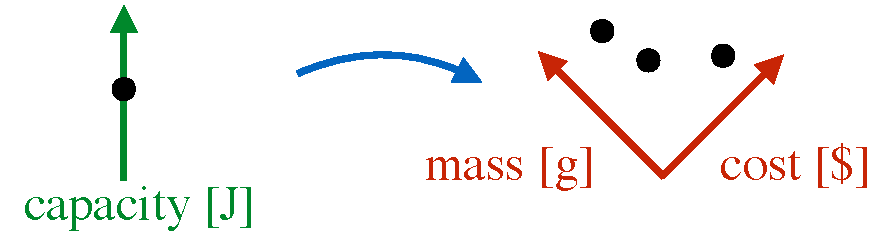
\includegraphics[scale=0.33]{reits2_battery2_h}}

A subset with ``minimal'', ``incomparable'' elements is called ``antichain''.
This is the mathematical formalization of what is informally called a ``Pareto front''.

%\begin{definition}\label{def:antichain-paper2}
%  An \emph{antichain}~$S$ in a poset~$\left\langle \posA,\posleq\right\rangle $
%  is a subset of~$\posA$ such that no element of~$S$ dominates another
%  element: if~$x,y\setin S$ and~$x\posleq y$, then~$x=y$.
%\end{definition}
%\begin{lemma}\label{lem:orderantichains}
%  Let~$\antichains\posA$ be the set of antichains of~$\posA$. $\antichains\posA$
%  is a poset itself, with the partial order~$\posleqof{\antichains\posA}$
%  defined as
%  \begin{equation}
%    S_{1}\posleqof{\antichains\posA}S_{2}\ \equiv\ \uparrow S_{1}\setsupseteq\,\uparrow S_{2}.\label{eq:orderantichains}
%  \end{equation}
%\end{lemma}
%\begin{definition}
%  \label{def:A-monotone-design}A\emph{ monotone design problem~}(DP)
%  is a tuple~$\left\langle \funsp,\ressp,\ftor\right\rangle $ such
%  that~$\funsp$ and~$\ressp$ are CPOs, and~${\colH\ftor}:{\colF\fun}\rightarrow{\colR\Aressp}$
%  is a monotone and Scott-continuous function~(\cite{gierz03continuous}
%  or \cite[Definition 11]{censi16codesign_sep16}).
%\end{definition}
\captionsideleft{}{\includegraphics[scale=0.33]{unc_ftor}}

Each functionality~\fun corresponds to an antichain of resources $\ftor(\fun)\setin\Aressp$~(\cref{fig:ftorgraph}).

\captionsideleft{\label{fig:ftorgraph}}{\includegraphics[scale=0.33]{unc_ftorgraph}}

Monotonicity implies that, if the functionality is increased, then the required resources increase as well~(\cref{fig:antichain2}).

\captionsideleft{\label{fig:antichain2}}{\includegraphics[scale=0.33]{unc_ftorgraph2}}

\section{Monotone Co-Design Problems }

A Monotone Co-Design Problem is a multigraph of DPs.
Two DPs can be connected by adding an edge~(\cref{fig:unc_connection}).
The semantics of the interconnection is that the resources required by the first DP must be provided by the second DP.
Mathematically, this is a partial order inequality constraint of the type~$\res_{1}\posleq\fun_{2}$.
Self-loops are allowed as well.

\captionsideleft{\label{fig:unc_connection}}{\includegraphics[scale=0.33]{unc_connection}}
%\begin{example}
%    The MCDP in~\cref{fig:example} is the interconnection of 3
%    DPs $\ftor_{a},\ftor_{b},\ftor_{c}.$ The semantics of the MCDP as
%    an optimization problem is shown in~\cref{fig:example-semantics}.
%\end{example}
%
%\captionsideleft{\label{fig:example}}{ \includegraphics[scale=0.33]{unc_atoms_g_v_graph}}\\
%\captionsideleft{\label{fig:example-semantics}}{\includegraphics[scale=0.33]{unc_semantics}}

To describe the interconnection, the obvious choice is to describe it as a graph, as a set of nodes and of edges.
For our goals, it is more convenient to use an algebraic definition.
In the algebraic definition, the graph is a represented by a tree, where the leaves are the nodes, and the junctions are one of three operators ($\dpseries,\dppar,\dploop$), as in~\cref{fig:series-par-loop}.

Similar constructions are widespread in computer science.
One can see this in the spirit of series-parallel graphs (see, \eg ,~\cite{duffin65topology}), with an additional feedback operator to be able to represent all graphs.
Equivalently, we are defining a symmetric traced monoidal category (see, \eg ,~\cite{joyal96traced} or~\cite{spivak14category} for an introduction); note that the~$\dploop$ operator is related to  the ``trace'' operator but not exactly equivalent, though they can be defined in terms of each other.
An equivalent construction for network processes is given in Stefanescu~\cite{stefanescu00}.

\begin{figure}[h]
    \centering{}\hfill{}\subfloat[$\dpseries(a,b)$]{\includegraphics[scale=0.33]{unc_dpseries}

    }\hfill{}\subfloat[$\dppar(a,b)$]{\includegraphics[scale=0.33]{unc_dppar}

    }\hfill{}\subfloat[$\dploop(a)$]{\includegraphics[scale=0.33]{unc_dploop}

    }\smallskip{}
    \caption{The three operators used in the inductive definition of MCDPs.}
    \label{fig:series-par-loop}
\end{figure}

Let us use a standard definition of ``operators'', ``terms'', and ``atoms'' (see, \eg~\cite[p.41]{jezek08}).
Given a set of operators~$\ops$ and a set of atoms~$\atoms$, let~$\terms(\ops,\atoms)$ be the set of all inductively defined expressions.
For example, if the operator set contains only an operator~$f$ of \emph{arity} 1, and there is only one atom~$a$, then the terms are $\terms(\makeset{f},\makeset{a})=\makeset{a,f(a),f(f(a)),\dots}.
$

\begin{definition}[Algebraic definition Monotone Co-Design Problems]
    \label{def:MCDP-algebraic}
    An MCDP is a tuple~$\left\langle \atoms,\atree,\val\right\rangle $,
    where:
    \begin{enumerate}
        \item $\atoms$ is any set of atoms, to be used as labels.
        \item The term~$\atree$ in the $\{\dpseries,\dppar,\dploop\}$ algebra
              describes the structure of the graph:
              \begin{equation}
                  \atree\setin\terms(\{\dpseries,\dppar,\dploop\},\atoms).
              \end{equation}
        \item The \emph{valuation} $\val$ is a map $\val:\atoms\rightarrow\dpsp$ that assigns a DP to each atom.
    \end{enumerate}
\end{definition}
\begin{example}
    \todotext{add reference}
    The MCDP in~\XXX can be described by the atoms
    $\atoms=\{a,b,c\}$, the term $\atree=\dploop(\dpseries(a,\dppar(b,c)),$
    plus the valuation $\val:\{a\mapsto\ftor_{a},b\mapsto\ftor_{b},c\mapsto\ftor_{c}\}.
    $
    The tuple~$\left\langle \atoms,\atree,\val\right\rangle $ for this
    example is shown in \cref{fig:example-b}.
\end{example}
\captionsideleft{\label{fig:example-b}}{\includegraphics[scale=0.33]{unc_atoms_g_v}}
\begin{example}
    A sketch of the algebraic representation for part of the example in~\cref{fig:Example1}
    is shown in~\cref{fig:tree2}.
    The supplementary materials contain
    more detailed visualizations of the trees for the numerical examples,
    which take too much space for including in this paper.
\end{example}
\captionsideleft{\label{fig:tree2}}{\includegraphics[scale=0.33]{unc_tree}}

\section{Semantics of MCDPs}

We can now define the \emph{semantics} of an MCDP.
The \emph{semantics} is a function~$\dpsem$ that, given an algebraic definition of an MCDP, returns a~$\dpsp$.
Thanks to the algebraic definition, to define~$\dpsem$, we need to only define what happens in the base case (equation~\ref{eq:base}), and what happens for each operator $\dpseries,\dppar,\dploop$ (\crefrange{eq:series}{eq:loop}).

\begin{definition}[Semantics of MCDP]
    \label{def:dpsem}
    Given an MCDP in algebraic form~$\left\langle \atoms,\atree,\val\right\rangle $, the semantics
    \begin{equation}
        \dpsem\llbracket\left\langle \atoms,\atree,\val\right\rangle \rrbracket\setin\dpsp
    \end{equation}
    is defined as follows:
    %
    \begin{align}
        \dpsem\llbracket\left\langle \atoms,a,\val\right\rangle \rrbracket                                & \definedas\val(a),\qquad\text{for all}\ a\setin\atoms,\label{eq:base} \\
        \dpsem\llbracket\left\langle \atoms,\dpseries(\atree_{1},\atree_{2}),\val\right\rangle \rrbracket & \definedas\dpsem\llbracket\left\langle \atoms,\atree_{1},\val\right\rangle \rrbracket\,\opseries\,\dpsem\llbracket\left\langle \atoms,\atree_{2},\val\right\rangle \rrbracket,\label{eq:series} \\
        \dpsem\llbracket\left\langle \atoms,\dppar(\atree_{1},\atree_{2}),\val\right\rangle \rrbracket    & \definedas\dpsem\llbracket\left\langle \atoms,\atree_{1},\val\right\rangle \rrbracket\,\oppar\,\dpsem\llbracket\left\langle \atoms,\atree_{2},\val\right\rangle \rrbracket,\label{eq:par} \\
        \dpsem\llbracket\left\langle \atoms,\dploop(\atree),\val\right\rangle \rrbracket                  & \definedas\dpsem\llbracket\left\langle \atoms,\atree,\val\right\rangle \rrbracket^{\oploop}.
        \label{eq:loop}
    \end{align}
\end{definition}
The operators $\opseries,\oppar,\oploop$ are defined in~\crefrange{def:opseries}{def:oploop}.
Please see~\cite[Section VI]{censi16codesign_sep16} for details about the interpretation of these operators and how they are derived.

The $\oppar$ operator is a regular product in category theory: we are considering all possible combinations of resources required by~$\ftor_{1}$ and~$\ftor_{2}$.
\begin{definition}
    [Product operator $\oppar$]
    \label{def:opmaps}
    For two maps $\ftor_{1}\colon\funsp_{1}\rightarrow\Aressp_{1}$
    and $\ftor_{2}\colon\funsp_{2}\rightarrow\Aressp_{2}$, define
    \begin{align*}
        \ftor_{1}\oppar\ftor_{2}:(\funsp_{1}\times\funsp_{2}) & \rightarrow\antichains(\ressp_{1}\times\ressp_{2}), \\
        \left\langle \fun_{1},\fun_{2}\right\rangle           & \mapsto\ftor_{1}(\fun_{1})\acprod\ftor_{2}(\fun_{2}),
    \end{align*}
    where $\acprod$ is the product of two antichains.
\end{definition}
The $\opseries$ operator is similar to a convolution: fixed $\fun_{1}$, one evaluates the resources $\res_{1}\setin\ftor_{1}(\fun)$, and for each~$\res_{1}$, $\ftor_{2}(\res_{1})$ is evaluated.
The $\Min$ operator then chooses the minimal elements.
\begin{definition}
    [Series operator~$\opseries$]
    \label{def:opseries}
    For two maps~$\ftor_{1}\colon\funsp_{1}\rightarrow\Aressp_{1}$
    and~$\ftor_{2}\colon\funsp_{2}\rightarrow\Aressp_{2}$, if~$\ressp_{1}=\funsp_{2}$
    , define
    \begin{align*}
        {\displaystyle \ftor_{1}\opseries\ftor_{2}\colon\funsp_{1}}
                  & \rightarrow\Aressp_{2}, \\
        \ftor_{1} & \mapsto\Min_{\posleqof{\ressp_{2}}}\bigsetunion_{\res_{1}\setin\ftor_{1}(\fun)}\ftor_{2}(\res_{1}).
    \end{align*}

\end{definition}

The dagger operator $\oploop$ is actually a standard operator used in domain theory (see, \eg ,~\cite[II-2.29]{gierz03continuous}).
\begin{definition}
    [Loop operator $\oploop$]
    \label{def:oploop}
    For a map $\ftor:\funsp_{1}\times\funsp_{2}\rightarrow\Aressp$,
    define
    \begin{align}
        \ftor^{\oploop}:\funsp_{1} & \rightarrow\Aressp,\nonumber \\
        \fun_{1}                   & \mapsto\lfp\left(\Psi_{\fun_{1}}^{\ftor}\right),
    \end{align}
    where $\lfp$ is the least-fixed point operator, and~$\Psi_{\fun_{1}}^{\ftor}$
    is defined as
    \begin{align*}
        \Psi_{\fun_{1}}^{\ftor}:\Aressp & \rightarrow\Aressp, \\
        {\colR R}                       & \mapsto\Min_{\posleqof{\ressp}}\bigsetunion_{\res\in{\colR R}}\ftor(\fun_{1},\res)\ \setintersection\uparrow\res.
    \end{align*}
\end{definition}

\section{Solution of MCDPs}

\Cref{def:dpsem} gives a way to evaluate the map~$\ftor$ for the graph, given the maps~$\{\ftor{}_{a}\mid a\setin\atoms\}$ for the leaves.
Following those instructions, we can compute~$\ftor(\fun)$, and thus find the minimal resources needed for the entire MCDP.
\begin{example}
    The MCDP in~\cref{fig:exampleq} is so small that we can do this explicitly.
    From~\cref{def:dpsem}, we can compute the semantics as follows:
    \begin{align*}
        \ftor & =\dpsem\left\llbracket \langle\atoms,\dploop(\dpseries(a,\dppar(b,c)),\val\rangle\right\rrbracket \\
              & =\left(\ftor_{a}\,\opseries\,\left(\ftor_{b}\,\oppar\,\ftor_{c}\right)\right)^{\oploop}.
    \end{align*}
    Substituting the definitions~\crefrange{def:opmaps}{def:oploop} above, one finds that $\ftor(\fun)=\lfp\left(\Psi_{\fun}\right),$ with
    \begin{align*}
        \Psi_{\fun}:\Aressp & \rightarrow\Aressp, \\
        {\colR R}           & \mapsto\bigsetunion_{\res\in{\colR R}}\Big[\Min_{\posleq}\uparrow\bigsetunion_{s\setin\ftor_{a}(\fun_{1},\res)}\ftor_{b}(s)\acprod\ftor_{c}(s)\Big]\ \setintersection\uparrow\res.
    \end{align*}
    The least fixed point equation can be solved using Kleene's algorithm~\cite[CPO Fixpoint theorem I, 8.15]{davey02}.
    A dynamical system that computes the set of solutions is given by
    \begin{equation}
        \begin{cases}
            {\colR R}
            _{0}            & \leftarrow\{\posbot_{\ressp}\},       \\
            {\colR R}_{k+1} & \leftarrow\Psi_{\fun}({\colR R}_{k}).
        \end{cases}
    \end{equation}
    The limit $\Sup{\colR R}_{k}$ is the set of minimal solutions, which might be an empty set if the problem is unfeasible.

    This dynamical system is a proper algorithm only if each step can be performed with bounded computation.
    An example in which this is not the case are relations that give an infinite number of solutions for each functionality.
    For example, the very first DP appearing in~\cref{fig:Example1} corresponds to the relation~${\colF\text{travel distance}}\leq{\colR\text{velocity}}\times{\colR\text{endurance}},$ for which there are infinite numbers of pairs~$\tupp{{\colR\text{velocity}},{\colR\text{endurance}}}$ for each value of~${\colF\text{travel distance}}$.
    The machinery developed in this paper will make it possible to deal with these infinite-cardinality relations by relaxation.
\end{example}

\section{Uncertain Design Problems}
\label{sec:UDP}

We now consider the introduction of uncertainty.
This section describes objects called Uncertain DPs (UDPs), which are an ordered pair of DPs.
Each pair can be interpreted as upper and lower bounds for resource consumptions~(\cref{fig:udp-bounds}).

\captionsideleft{\label{fig:udp-boundsOLD}}{\includegraphics[scale=0.33]{unc_ftorLU}}

We will be able to propagate this interval uncertainty through an arbitrary interconnection of DPs.
The result presented to the user will be a \emph{pair} of antichains \textemdash{} a lower and an upper bound for the resource consumption.

\section{Partial order $\dpleq$}

Being able to provide both upper and lower bounds comes from the fact that in this framework everything is ordered---there are a poset of resources, lifted to posets of antichains, which is lifted  to posets of DPs, and finally, to the poset of uncertain DPs.

The first step is defining a partial order~$\dpleq$ on~$\dpsp$.
\begin{definition}
    [Partial order $\dpleq$]
    Consider two DPs $\ftor_{1},\ftor_{2}:\funsp\rightarrow\Aressp$.
    The DP~$\ftor_{1}$ precedes~$\ftor_{2}$ if it requires fewer resources
    for all functionality~\fun:
    \begin{equation}
        \ftor_{1}\dpleq\ftor_{2}\quad\equiv\quad\ftor_{1}(\fun)\posleqof{\Aressp}\ftor_{2}(\fun),\ \text{for all }\fun\setin\funsp.
    \end{equation}
\end{definition}

\captionsideleft{}{\includegraphics[scale=0.33]{unc_dporder}\includegraphics[scale=0.33]{unc_dpleq2}}

In this partial order, there is both a top~$\postop_{\dpsp}$ and a bottom~$\posbot_{\dpsp}$, defined as follows:

\vspace{-5mm}

\begin{minipage}[t]{0.4\columnwidth}
    \begin{align*}
        \posbot_{\dpsp}:\funsp & \rightarrow\Aressp, \\
        \fun                   & \mapsto\{\posbot_{\ressp}\}.
    \end{align*}

\end{minipage}
\begin{minipage}[t]{0.4\columnwidth}
    \begin{align}
        \postop_{\dpsp}:\funsp & \rightarrow\Aressp,\nonumber \\
        \fun                   & \mapsto\Emptyset.\label{eq:top}
    \end{align}

\end{minipage}

$\posbot_{\dpsp}$~means that any functionality can be done with zero resources, and~$\postop_{\dpsp}$ means that the problem is always infeasible (``the set of feasible resources is empty'').

\section{Uncertain DPs (UDPs)}
\begin{definition}[Uncertain DPs]
    An Uncertain DP (UDP)~$\boldsymbol{u}$ is a pair of DPs~$\langle\udpL\boldsymbol{u},\udpU\boldsymbol{u}\rangle$
    such that~$\udpL\boldsymbol{u}\dpleq\udpU\boldsymbol{u}$.
\end{definition}
\captionsideleft{}{\includegraphics[scale=0.33]{unc_udpdef}}

\section{Order on UDP}
\begin{definition}
    [Partial order $\udpleq$]
    A UDP~$\udpa$ precedes another UDP~$\udpb$ if the interval~$[\udpL\udpa,\udpU\udpa]$ is contained in the interval~$[\udpL\udpa,\udpU\udpa]$ (\cref{fig:udpspace}):
    \begin{equation}
        \udpa\udpleq\udpb\quad\equiv\quad\udpL\udpb\dpleq\udpL\udpa\dpleq\udpU\udpa\dpleq\udpU\udpb.
    \end{equation}
\end{definition}
\captionsideleft{\label{fig:udpspaceOLD}}{\includegraphics[scale=0.33]{unc_udpab2}\includegraphics[scale=0.33]{unc_udpab}}

The partial order~$\udpleq$ has a top~$\postop_{\udpsp}=\left\langle \posbot_{\dpsp},\postop_{\dpsp}\right\rangle.
$
This pair describes maximum uncertainty about the DP: we do not know if the DP is feasible with 0 resources~($\posbot_{\dpsp}$), or if it is completely infeasible~($\postop_{\dpsp}$).

\section{DPs as degenerate UDPs}

A DP~$\ftor$ is equivalent to a degenerate UDP~$\langle\ftor,\ftor\rangle$.

A UDP~$\boldsymbol{u}$ is a bound for a DP~$\ftor$ if~$\boldsymbol{u}\udpleq\langle\ftor,\ftor\rangle$,
or, equivalently, if $\udpL\boldsymbol{u}\udpleq\ftor\udpleq\udpU\boldsymbol{u}$.

\captionsideleft{\label{fig:pyr1OLD}}{\hspace{-9mm}\includegraphics[scale=0.33]{unc_dpcones2}\includegraphics[scale=0.33]{unc_dpcones}}

A pair $\langle\ftor,\ftor\rangle$ is a minimal element of~$\udpsp$, because it cannot be dominated by any other.
Thus, we can imagine the space $\udpsp$ as a pyramid~(\cref{fig:pyr1}), with the space~$\dpsp$ forming the base.
The base represents non-uncertain DPs.
The top of the pyramid is~$\postop_{\udpsp}$, which represents maximum uncertainty.

\section{Interconnection of Uncertain Design Problems\label{sec:UMCDP}}

We now define the interconnection of UDPs, in an equivalent way to the definition of MCDPs.
The only difference between \cref{def:MCDP-algebraic} and~\cref{def:umcdp} below is that the valuation assigns to each atom an UDP, rather than a~DP.
\begin{definition}[Algebraic definition of UMCDPs]
    \label{def:umcdp}
    An Uncertain MCDP (UMCDP) is a tuple~$\left\langle \atoms,\atree,\val\right\rangle$, where~$\atoms$ is a set of atoms, $\atree\setin\terms(\{\dpseries,\dppar,\dploop\},\atoms)$ is the algebraic representation of the graph, and~$\val:\atoms\rightarrow\udpsp$ is a valuation that assigns to each atom a UDP.
\end{definition}

Next, the semantics of a UMCDP is defined as a map~$\udpsem$ that computes the UDP.
\Cref{def:semantics-udp}~below is analogous to~\cref{def:dpsem}.

\begin{definition}[Semantics of UMCDPs]
    \label{def:semantics-udp}
    Given an UMCDP~$\left\langle \atoms,\atree,\val\right\rangle $,
    the semantics function~$\udpsem$ computes a UDP
    \begin{equation}
        \udpsem\llbracket\left\langle \atoms,\atree,\val\right\rangle \rrbracket\setin\udpsp,
    \end{equation}
    and it is recursively defined as follows:
    \begin{equation}
        \udpsem\llbracket\left\langle \atoms,a,\val\right\rangle \rrbracket=\val(a),\qquad\text{for all}\ a\setin\atoms.
    \end{equation}
    \begin{align*}
        \udpL\udpsem\llbracket\left\langle \atoms,\dpseries(\atree_{1},\atree_{2}),\val\right\rangle \rrbracket & =(\udpL\udpsem\llbracket\left\langle \atoms,\atree_{1},\val\right\rangle \rrbracket)\,\opseries\,(\udpL\udpsem\llbracket\left\langle \atoms,\atree_{2},\val\right\rangle \rrbracket), \\
        \udpU\udpsem\llbracket\left\langle \atoms,\dpseries(\atree_{1},\atree_{2}),\val\right\rangle \rrbracket & =(\udpU\udpsem\llbracket\left\langle \atoms,\atree_{1},\val\right\rangle \rrbracket)\,\opseries\,(\udpU\udpsem\llbracket\left\langle \atoms,\atree_{2},\val\right\rangle \rrbracket),
    \end{align*}
    \begin{align*}
        \udpL\udpsem\llbracket\left\langle \atoms,\dppar(\atree_{1},\atree_{2}),\val\right\rangle ] & =(\udpL\udpsem\llbracket\left\langle \atoms,\atree_{1},\val\right\rangle \rrbracket)\ \oppar\ (\udpL\udpsem\llbracket\left\langle \atoms,\atree_{2},\val\right\rangle \rrbracket), \\
        \udpU\udpsem\llbracket\left\langle \atoms,\dppar(\atree_{1},\atree_{2}),\val\right\rangle ] & =(\udpU\udpsem\llbracket\left\langle \atoms,\atree_{1},\val\right\rangle \rrbracket)\ \oppar\ (\udpU\udpsem\llbracket\left\langle \atoms,\atree_{2},\val\right\rangle \rrbracket),
    \end{align*}
    \begin{align*}
        \udpL\udpsem\llbracket\left\langle \atoms,\dploop(\atree),\val\right\rangle \rrbracket & =(\udpL\udpsem\llbracket\left\langle \atoms,\atree,\val\right\rangle \rrbracket)^{\oploop}, \\
        \udpU\udpsem\llbracket\left\langle \atoms,\dploop(\atree),\val\right\rangle \rrbracket & =(\udpU\udpsem\llbracket\left\langle \atoms,\atree,\val\right\rangle \rrbracket)^{\oploop}.
    \end{align*}

\end{definition}
The operators $\oploop,\opseries,\oppar$ are defined in \crefrange{def:opseries}{def:oploop}.

The rest of the paper consists of applications of this result.
